\documentclass[14pt]{extarticle}
\usepackage{amssymb,amsthm,amsmath, color}
\usepackage{graphicx}
\usepackage{float}
\usepackage{fullpage}
\usepackage{subfigure}
\usepackage{graphics}

\newtheorem{theorem}{Theorem}[section]
\newtheorem{lemma}[theorem]{Lemma}
\newtheorem{proposition}[theorem]{Proposition}
\newtheorem{claim}[theorem]{Claim}
\newtheorem{corollary}[theorem]{Corollary}
\newtheorem{definition}[theorem]{Definition}
\newtheorem{observation}[theorem]{Observation}
\newtheorem{fact}[theorem]{Fact}
\newtheorem{property}{Property}
\newtheorem{remark}{Remark}[section]
\newtheorem{notation}{Notation}[section]
\newtheorem{example}{Example}[section]
\newtheorem{algorithm}{Algorithm}
\newtheorem{conjecture}{Conjecture}
\newtheorem{question}[conjecture]{Question}

\newcommand{\Z}{\mathbb{Z}} 

\begin{document}
\section*{CSE 2321 Homework 3 Template}
%This is a template file to make it easier for you to nicely writeup and submit your homework. For each problem I have put an example below with comments on how to nicely format your answers. If you have any trouble with this file or figuring out the format, please post on Piazza.


\subsection*{1}
\begin{itemize}
\item $|Pow(A)| = $
16
\item $Pow(A) = \{ \}$, 
$\{1 \}$, $\{2 \}$, $\{3 \}$, $\{6 \}$, $\{1,2 \}$, $\{ 1,3\}$, $\{ 1,6\}$, $\{ 2,3\}$, $\{2,6 \}$, $\{3,6 \}$, $\{1,2,3 \}$, $\{1,2,6 \}$, $\{1,3,6 \}$, $\{2,3,6 \}$, $\{1,2,3,6 \}$
\item $|Pow(A \cup B)| = $
32
\item $|Pow(A \cap B)| = $
8
\item $Pow(A \setminus B) = \{  \}$, $\{ 1\}$
\end{itemize}

\subsection*{2}
\begin{itemize}
\item The set of even numbers $ = \{ x \in \mathbb{N} : \exists y \in \mathbb{N}, x \div 2 = y \}$ 
\item The set of prime numbers $ = \{x \in \mathbb{N}  : \exists a,b \in \mathbb{N}, (a \geq 1) \land (b \geq a), a * b = x \iff (a = 1) \land (b = x)  \}$
\end{itemize}

\subsection*{3}
\begin{align*}
A &= \{3, 4, 5, 6 \} \\
B &= \{ 1, 2, 3, 4 \} \\
X &= \{1, 2, 3, 4, 5, 6  \} \\
Y &= \{4, 5, 6, 7, 8, 9  \} \\
Z &= \{2, 4, 6  \}
\end{align*}

\subsection*{4}
% This allows you to include pictures 
% Remove the '%' character from in front of \includegraphics 
% and replace figure_1.png with the name of your file, which
% must be contained in the same folder as this template file
\begin{figure}[H]
\centering
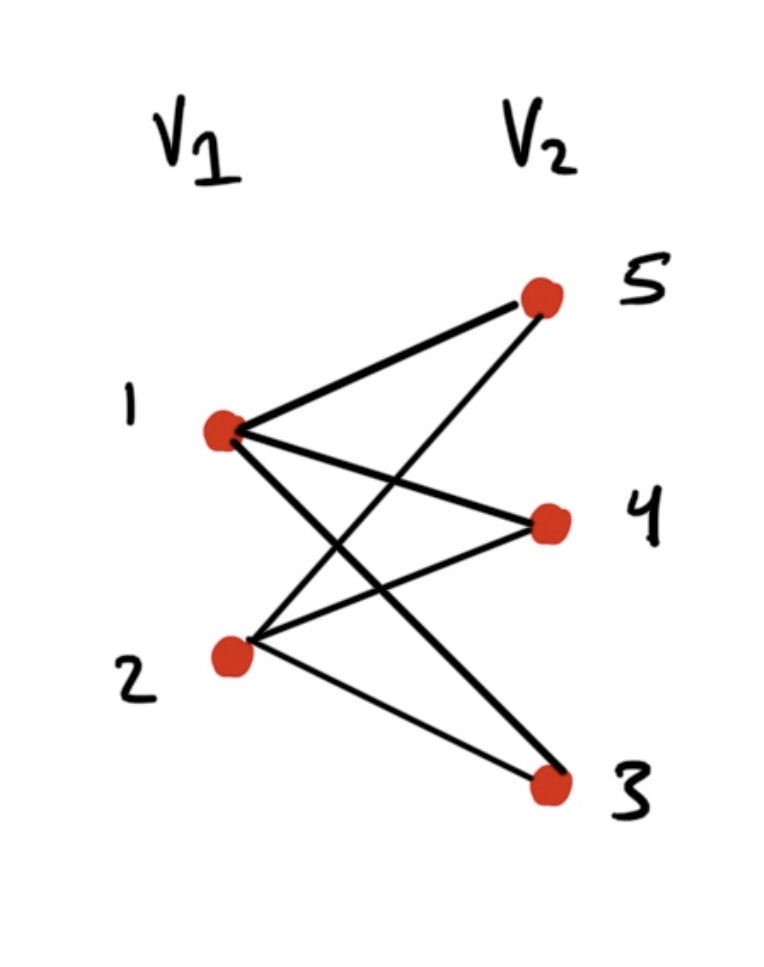
\includegraphics[width=0.5\textwidth]{bitartite.png}
\end{figure}

\subsection*{5}
%You can just list the vertices here:
4, 2, 3, 5, 4, 1, 3, 6, 4, 8, 3, 12, 4



\subsection*{6}

\begin{align*}
\sum_{i=1}^{n} \frac{1}{i(i+1)} = \frac{n}{n+1} 
\end{align*}
\begin{proof}[Proof By Induction]\hfill \\
\emph{Base Case:}\\
Let n = 1 \\
$\sum_{i=1}^{n} \frac{1}{i(i+1)} = \frac{n}{n+1} \\ = \frac{1}{i(i+1)} = \frac{1}{1(1+1)} = \frac{1}{2} \\ = \frac{1}{i + 1} = \frac{n}{n + 1} $ \\
\emph{Induction Step:}\\
Let n be an arbitrary number and assume, \\

$\sum_{i=1}^{n} \frac{1}{i(i+1)} = \frac{n}{n + 1} $ , so \\\\
$\sum_{i=1}^{n+1} \frac{1}{i(i+1)} = \frac{n+1}{n + 1+1} $, so \\\\
$\sum_{i=1}^{n+1} \frac{1}{i(i+1)} = \sum_{i=1}^{n} \frac{1}{i(i+1)} + \frac{n+1}{(n+1)(n+1+1)}$ \\\\
$= \frac{n}{n+1} + \frac{n+1}{(n+1)(n+2)} = \frac{n(n+2) + (n+1)}{(n+1)(n+2)} $
 \\\\
 $= \frac{n}{n+1} + \frac{1}{n+2}$ \\
 $= \sum_{i=1}^{n} \frac{1}{i(i+1)} + \frac{1}{n+2}$\\
 

% & specifies what each line should be aligned on
% \\ creates a newline
\emph{Conclusion:}\\
\end{proof}
$\sum_{i=1}^{n} \frac{1}{i(i+1)} = \frac{n}{n+1}$ \\


\end{document}
